\subsection{Further Reducing the Input Size}

The size of input is determined by the dimension of inputs (originally \(16 \times 16\)) and the depth of each pixel (8-bit in the previous section).
A search is done as \autoref{fig:mnist-shrink} to find a suitable pair of dimension and depth with the naive linear regression model.


When the input size is shrunk to \(8 \times 8\), the misclassifications rate is 15.96\%, which is slightly worse than our target (over 85\% in accuracy).
However, this is a desirable configuration, which means we can fit an input in precisely 8 bytes.
Thus I believe it is worth sacrificing some accuracy here and getting it back using a more aggressive model.

\begin{figure}[ht!]
    \centering
    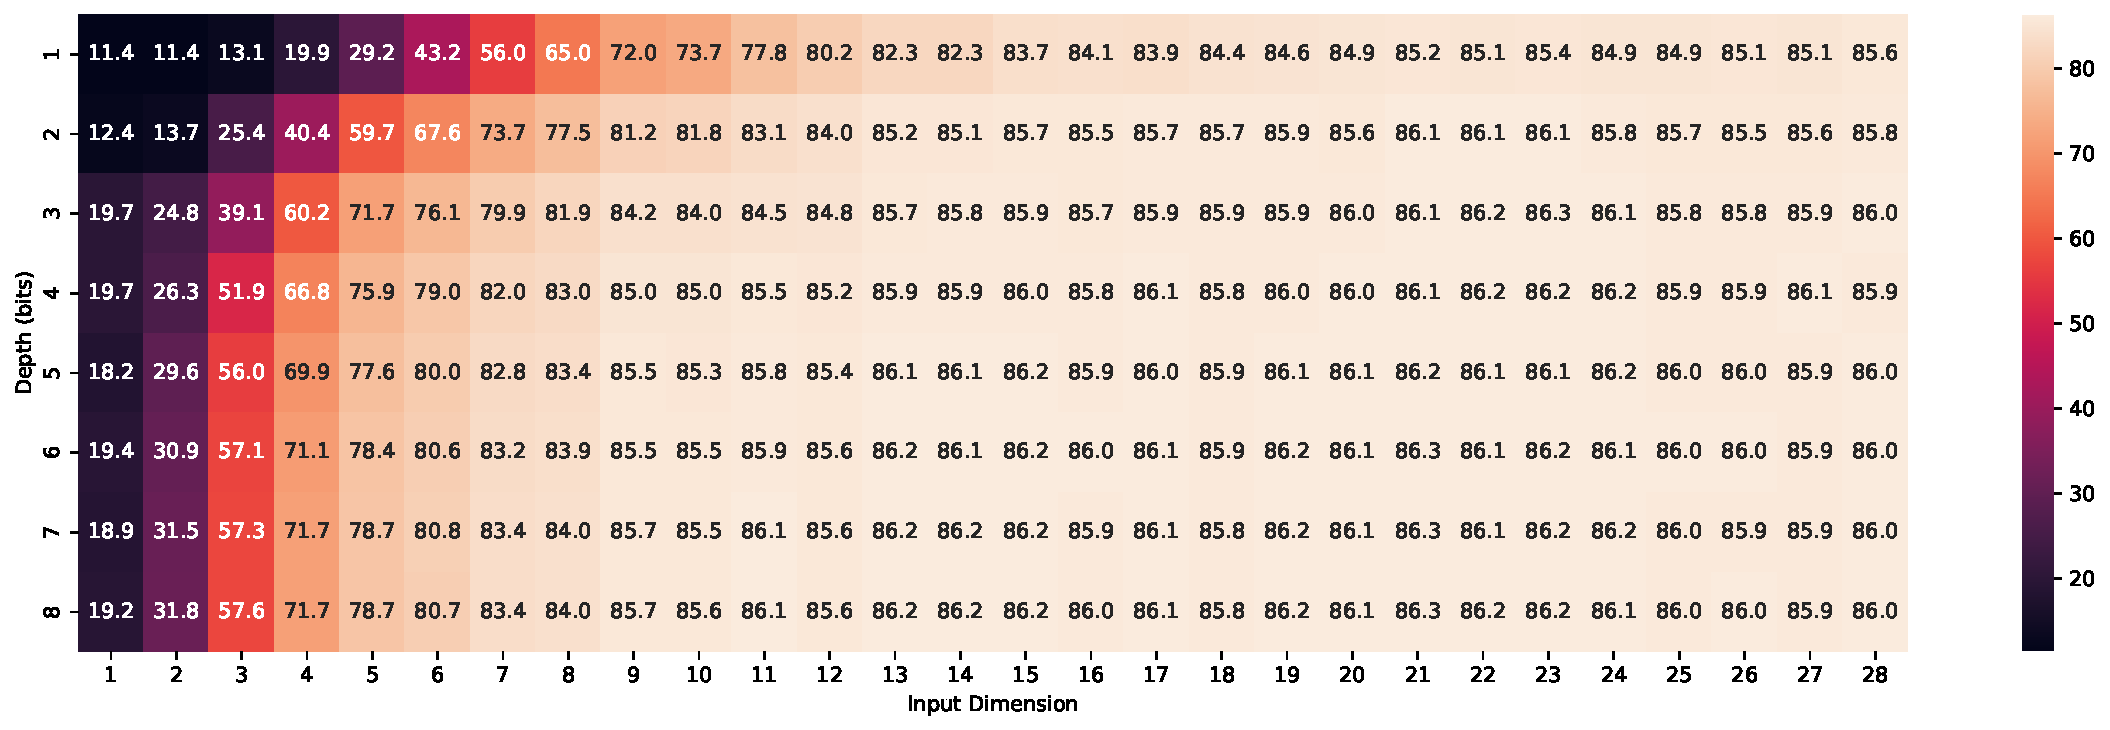
\includegraphics[width=\textwidth]{images/mnist-shrink.pdf}
    \caption{Prediction accuracy with floating point numbers under different input size}
    \label{fig:mnist-shrink}
\end{figure}


Grading breakdown

\begin{itemize}
    \item You will receive full marks if you can both improve performance and accuracy of your classifier by a significant margin (\textbf{over 85\% in accuracy, and achieve less than 4.5ms of FPGA inference time} as measured on the board for 8k invocations). You are free to change the classifier algorithm.
    \item The best projects will include ambitious classifier implementations (e.g. neural networks).
\end{itemize}

Hints To provide some guidance, you can implement one of the following optimizations:

\begin{itemize}
    \item \textbf{Image resizing} to reduce bandwidth constraints
    \item \textbf{Int4} computation to improve overall throughput and compute parallelism
    \item Static weight and input pruning to improve throughput
    \item Tweaking the classifier parameters (alpha, normalize, solver etc.) to minimize the impact of quantization after training: \url{http://scikit-learn.org/stable/modules/generated/sklearn.linear_model.RidgeClassifier.html}
    \item Quantized training of Perceptrons or MLPs to greatly improve on accuracy (hard): you can try using Tensorflow's quantized neural network training framework based on Google's gemmlowp
\end{itemize}
